\documentclass[a4paper,12pt]{article}
\usepackage[utf8]{inputenc}
\usepackage{calc}
\usepackage{eso-pic}
\usepackage{graphicx}
\usepackage{parskip}
\usepackage{hyperref}
\usepackage[a4paper,left=25 mm,right=25 mm, bottom=25 mm,
    margin=1in,top=22 mm]{geometry} % Adjusting the margins
\usepackage{tikz}
\usepackage{array}
\usepackage{tabularx}
\usepackage{amsmath}
\usepackage{amssymb}
\usetikzlibrary{calc}

\begin{document}

\begin{titlepage}
\begin{tikzpicture}
    [remember picture, overlay]
    \draw[line width = 2pt, black] 
        ($(current page.north west) + (1cm,-1cm)$) 
        rectangle 
        ($(current page.south east) + (-1cm,1cm)$);
\end{tikzpicture}
    \centering
    \vspace*{0 cm}
    \Large
    \textbf{Maulana Abul Kalam Azad University of Technology, WB}
    \vspace{0.5cm}
    
    
\includegraphics[width=0.3\textwidth]{306-3063564_maulana-abul-kalam-azad-university-logo.png} % Assuming you have the logo image
    \vspace{0.5cm}
    
    \LARGE
    \textbf{\textcolor{blue!60}{Software Tools and Technology\\
        -: Lab Notebook :-}}
    \vspace{0.5cm}
    
    \large
    \textbf{\textcolor{red}{Group 13}}
    \vspace{1 cm}
    
    \textbf{Repository Link:} \href{https://github.com/mishbah-ul-haque/GROUP--13}{https://github.com/mishbah-ul-haque/GROUP--13}
    \vspace{1cm}
    
    \textbf{\underline{\textcolor{blue!60}{Group Members}}}
    \vspace{0.5cm}

    \normalsize
    \begin{enumerate}
        \item \textbf{Sk Mishbah Ul Haque(Leader)}\\
              \textbf{Roll No: 30001223058}\\
              \textbf{Department: BCA}
        \item \textbf{Md Nasim Akhtar}\\
              \textbf{Roll No: 30001223064}\\
              \textbf{Department: BCA}
        \item \textbf{Sreyash Anand}\\
              \textbf{Roll No: 30001223006}\\
              \textbf{Department: BCA}
        \item \textbf{Ritesh Kumar Shah}\\
              \textbf{Roll No: Ritesh Kumar Shah}\\
              \textbf{Department: BCA}
        \item \textbf{Sayantani Hansda}\\
              \textbf{Roll No: 30054623020}\\
              \textbf{Department: BSc in IT (Data Science)}
    \end{enumerate}
    \vspace{0.8 cm}
    
    \textbf{Instructor:} \href{mailto:ayan.ghosh@university.edu}{\textcolor{blue}{Ayan Ghosh}}\\
    \vspace{0.2cm}
    
    \textbf{\textit{Date: September 11, 2024}}

\end{titlepage}
\newpage
\begin{tikzpicture}
    [remember picture, overlay]
    \draw[line width = 2pt, black]
        ($(current page.north west) + (1cm,-1cm)$)
        rectangle 
        ($(current page.south east) + (-1cm,1cm)$);
\end{tikzpicture}
\vspace{-2cm}

\centering
\section*{\underline{\Huge\textbf{\textcolor{blue!60}{Index}}}}
\vspace{0.5cm}

\renewcommand{\arraystretch}{2}
\setlength{\tabcolsep}{0pt} 

\begin{tabular}{|>{\centering\arraybackslash}p{80pt}|>{\centering\arraybackslash}p{350pt}|}
\hline
\textbf{Serial No.} & \textbf{Questions} \\
\hline
1 & Introduction to GitHub and GitHub Desktop version installation \\\hline
2 & Building a C program for a calculator in the local repository,committing,and publishing it as a public repository \\\hline
3 & Converting a submit button to Chin Tapak Dum Dum \\\hline
4 & Building CV in LaTeX \\\hline
5 & Branching and Merging \\\hline

\end{tabular}

\newpage
\begin{tikzpicture}
    [remember picture, overlay]
    \draw[line width = 2pt, black] 
        ($(current page.north west) + (1cm,-1cm)$) 
        rectangle 
        ($(current page.south east) + (-1cm,1cm)$);
\end{tikzpicture}
\vspace{-2cm}
% Lab notebook entries
\section*{\Huge{\textcolor{blue!60}{Lab Notebook Entries}}}

\subsection*{Entry by Sk Mishbah Ul Haque}
\textit{Date: [\today]}\\
\vspace{1 cm}
\begin{figure}[h!]
   \centering
    
\includegraphics[width=0.5\linewidth]{25231.png}
\end{figure}
\vspace{0.5 cm}

\section*{\Huge{\underline{{-:GitHub:-}}}}
\paragraph{\noindent}{GitHub is a web-based platform that allows developers to host, share, and collaborate on software projects. It provides a version control system powered by Git, enabling teams to track changes, manage code repositories, and work together seamlessly across different locations. GitHub supports collaborative development through features like pull requests, issues, and project boards, making it essential for open-source projects and professional software development. Additionally, it integrates with various development tools, enhancing productivity and streamlining the software development lifecycle.}

\subsection*{\underline{-:Installation:-}}
\paragraph{\setlength{\parindent}{0pt}}{Installing GitHub Desktop is a straightforward process that enhances your workflow by providing a user-friendly interface for managing repositories. To begin, download the installer from the [official GitHub Desktop website](https://desktop.github.com/) for your operating system—Windows or macOS. After downloading, run the installer and follow the on-screen instructions to complete the setup. Once installed, launch the application and sign in with your GitHub credentials, or create a new account if needed. GitHub Desktop simplifies the process of cloning repositories, making commits, and managing branches, making it an invaluable tool for developers of all skill levels. For Linux users, alternative methods like using Wine or other Git clients are available.}

\subsection*{Entry by Md Nasim Akhtar}
\textit{Date: [\today]}\\


\section*{Creating a GitHub Repository and C Calculator Program}

\subsection*{Step 1: Download and Install GitHub Desktop}
1. Go to the GitHub Desktop Website: Visit \texttt{https://desktop.github.com/} and download the installer for your OS.\\
2. Install the Application: Run the installer and follow the instructions.\\
3. Log In: Open GitHub Desktop and log in with your GitHub account.

\subsection*{Step 2: Go Through the Tutorial}
1. After logging in, GitHub Desktop may prompt you for a tutorial.\\
2. Pay attention to how to publish a repository.

\subsection*{Step 3: Create a Local Repository}
1. Click on \texttt{File} and choose \texttt{New Repository}.\\
2. Fill in repository details: 
   \begin{itemize}
       \item Name: e.g., \texttt{C-Calculator}.
       \item Local Path: Choose a location.
   \end{itemize}
3. Click \texttt{Create Repository}.

\subsection*{Step 4: Write a Simple C Program for a Calculator}

\vspace{1 cm}
\begin{figure}[h!]
   \centering
    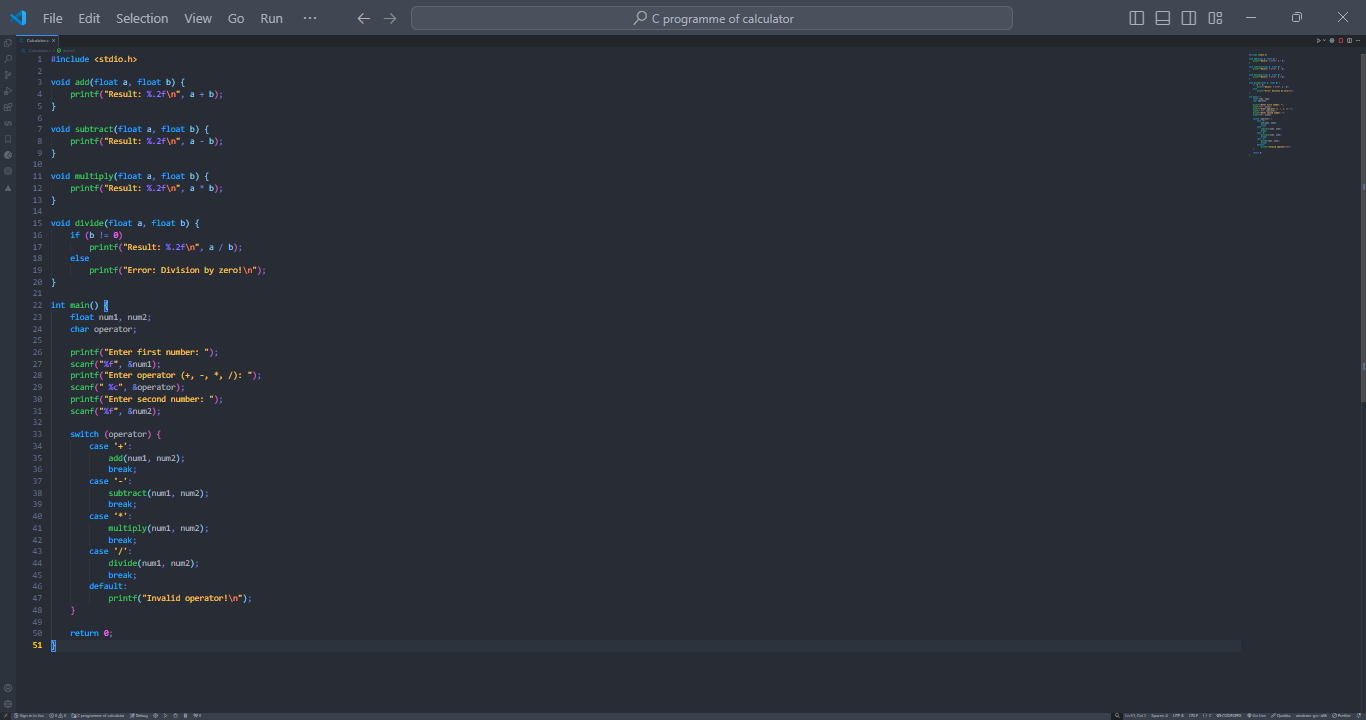
\includegraphics[width=0.5\linewidth]{C-calulator.png}
\end{figure}
\vspace{0.5 cm}

\subsection*{Step 5: Commit the Changes in GitHub Desktop}
1. View changes and enter a commit message.\\
2. Click \texttt{Commit to main}.

\subsection*{Step 6: Publish the Repository}
1. Click \texttt{Publish repository}.\\
2. Choose visibility (public or private).\\
3. Click \texttt{Publish Repository}.

\subsection*{Entry by Sreyash Anand}
\textit{Date: [\today]}\\
% Write your lab notebook entry here.

\subsection*{Entry by Ritesh Kumar Shah}
\textit{Date: [\today]}\\
% Write your lab notebook entry here.

\subsection*{Entry by Sayantani Hansda}
\textit{Date: [\today]}\\
% Write your lab notebook entry here.


\end{document}
